\documentclass[tikz,border=4pt]{standalone}
\usepackage{tikz}
\usetikzlibrary{shapes.geometric, arrows.meta, positioning, fit, backgrounds, calc}

% ─────────────────────────────────────────────────────────────────────────────
% Figure 1 — P7 Workflow Schematic
%
% Pipeline: ANP Library → SMILES → ECFP4 fingerprints → Classical encoder
%           → Quantum circuit (4-qubit QFE) → Decoder → Activity prediction
%
% Three evaluation phases shown as a row at the bottom.
% ─────────────────────────────────────────────────────────────────────────────

% Colour palette (colour-blind safe, matches matplotlib figures)
\definecolor{colANP}    {RGB}{33,102,172}   % blue   — data/input
\definecolor{colClassic}{RGB}{140,81,10}    % brown  — classical block
\definecolor{colQML}    {RGB}{214,96,77}    % red    — quantum block
\definecolor{colOut}    {RGB}{35,139,69}    % green  — output
\definecolor{colPhase}  {RGB}{117,112,179}  % purple — evaluation phases
\definecolor{colBg}     {RGB}{247,247,247}  % light grey background

\tikzset{
  % Main pipeline nodes
  datanode/.style={
    rectangle, rounded corners=3pt,
    draw=colANP!80, fill=colANP!12, thick,
    text width=2.0cm, align=center,
    font=\small\sffamily, inner sep=5pt, minimum height=1.0cm
  },
  classicnode/.style={
    rectangle, rounded corners=3pt,
    draw=colClassic!80, fill=colClassic!10, thick,
    text width=2.0cm, align=center,
    font=\small\sffamily, inner sep=5pt, minimum height=1.0cm
  },
  qnode/.style={
    rectangle, rounded corners=3pt,
    draw=colQML!80, fill=colQML!12, thick,
    text width=2.2cm, align=center,
    font=\small\sffamily, inner sep=5pt, minimum height=1.0cm
  },
  outnode/.style={
    rectangle, rounded corners=5pt,
    draw=colOut!80, fill=colOut!12, thick,
    text width=2.0cm, align=center,
    font=\small\sffamily\bfseries, inner sep=5pt, minimum height=1.0cm
  },
  phasenode/.style={
    rectangle, rounded corners=3pt,
    draw=colPhase!70, fill=colPhase!10,
    text width=2.8cm, align=center,
    font=\footnotesize\sffamily, inner sep=4pt, minimum height=0.9cm
  },
  % Arrows
  mainarrow/.style={
    -{Stealth[length=5pt,width=4pt]},
    thick, color=black!55
  },
  phasearrow/.style={
    -{Stealth[length=4pt,width=3pt]},
    thick, color=colPhase!70, dashed
  },
  % Labels on arrows
  arrowlabel/.style={font=\scriptsize\sffamily, color=black!55,
                      fill=white, inner sep=1.5pt}
}

\begin{document}
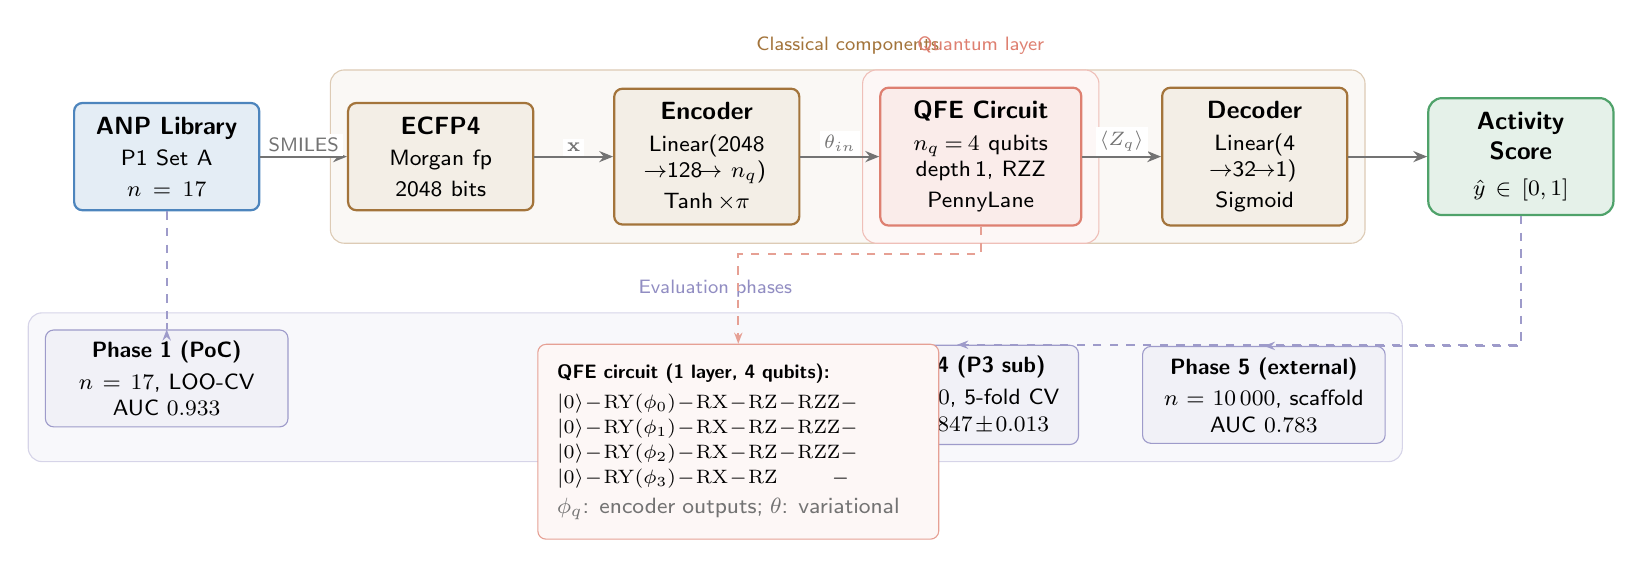
\begin{tikzpicture}[node distance=0.55cm and 0.45cm]

% ── Row 1: main pipeline ──────────────────────────────────────────────────────

\node[datanode] (anp) {
  \textbf{ANP Library}\\[2pt]
  {\footnotesize P1 Set A\\$n=17$}
};

\node[classicnode, right=1.1cm of anp] (ecfp4) {
  \textbf{ECFP4}\\[2pt]
  {\footnotesize Morgan fp\\2048 bits}
};

\node[classicnode, right=1.0cm of ecfp4] (encoder) {
  \textbf{Encoder}\\[2pt]
  {\footnotesize Linear(2048\\$\!\to$128$\!\to n_q$)\\Tanh$\,\times\pi$}
};

\node[qnode, right=1.0cm of encoder] (circuit) {
  \textbf{QFE Circuit}\\[2pt]
  {\footnotesize $n_q\!=\!4$ qubits\\depth\,1, RZZ\\PennyLane}
};

\node[classicnode, right=1.0cm of circuit] (decoder) {
  \textbf{Decoder}\\[2pt]
  {\footnotesize Linear(4\\$\!\to$32$\!\to$1)\\Sigmoid}
};

\node[outnode, right=1.0cm of decoder] (pred) {
  \textbf{Activity}\\
  \textbf{Score}\\[2pt]
  {\footnotesize $\hat{y}\in[0,1]$}
};

% Main pipeline arrows
\draw[mainarrow] (anp)     -- node[arrowlabel, above] {SMILES}   (ecfp4);
\draw[mainarrow] (ecfp4)   -- node[arrowlabel, above] {$\mathbf{x}$}     (encoder);
\draw[mainarrow] (encoder) -- node[arrowlabel, above] {$\theta_\text{in}$} (circuit);
\draw[mainarrow] (circuit) -- node[arrowlabel, above] {$\langle Z_q\rangle$} (decoder);
\draw[mainarrow] (decoder) -- node[arrowlabel, above] {} (pred);

% ── Row 2: evaluation phases ──────────────────────────────────────────────────

\node[phasenode, below=1.5cm of anp] (p1) {
  \textbf{Phase 1 (PoC)}\\[2pt]
  $n=17$, LOO-CV\\
  AUC $0.933$
};

\node[phasenode, below=1.5cm of circuit, xshift=-0.3cm] (p4) {
  \textbf{Phase 4 (P3 sub)}\\[2pt]
  $n=1000$, 5-fold CV\\
  AUC $0.847\!\pm\!0.013$
};

\node[phasenode, right=0.8cm of p4] (p5) {
  \textbf{Phase 5 (external)}\\[2pt]
  $n=10\,000$, scaffold\\
  AUC $0.783$
};

% Vertical dashed connectors from pipeline to phases
\draw[phasearrow] (anp.south)     |- (p1.north);
\draw[phasearrow] (pred.south)    |- (p4.north);
\draw[phasearrow] (pred.south)    |- (p5.north);

% ── Quantum circuit zoom-in box ───────────────────────────────────────────────

\node[below=1.5cm of encoder, xshift=0.4cm,
      draw=colQML!60, fill=colQML!5,
      rounded corners=3pt, inner sep=7pt,
      text width=4.6cm, align=left,
      font=\scriptsize\sffamily] (zoom) {
  \textbf{QFE circuit (1 layer, 4 qubits):}\\[3pt]
  $|0\rangle\!-\!\mathrm{RY}(\phi_0)\!-\!\mathrm{RX}\!-\!\mathrm{RZ}\!-\!\mathrm{RZZ}-$\\[1pt]
  $|0\rangle\!-\!\mathrm{RY}(\phi_1)\!-\!\mathrm{RX}\!-\!\mathrm{RZ}\!-\!\mathrm{RZZ}-$\\[1pt]
  $|0\rangle\!-\!\mathrm{RY}(\phi_2)\!-\!\mathrm{RX}\!-\!\mathrm{RZ}\!-\!\mathrm{RZZ}-$\\[1pt]
  $|0\rangle\!-\!\mathrm{RY}(\phi_3)\!-\!\mathrm{RX}\!-\!\mathrm{RZ}\!\quad\quad\quad\!-$\\[3pt]
  {\footnotesize\color{black!55}$\phi_q$: encoder outputs; $\theta$: variational}
};

% Connector from circuit node to zoom box
\draw[phasearrow, color=colQML!60]
  (circuit.south) -- ++(0,-0.35) -| (zoom.north);

% ── Background fit boxes for groups ──────────────────────────────────────────

\begin{pgfonlayer}{background}
  % Classical group
  \node[fit=(ecfp4)(encoder)(decoder),
        draw=colClassic!30, fill=colClassic!4,
        rounded corners=5pt, inner sep=6pt,
        label={[font=\scriptsize\sffamily\color{colClassic!80},
                yshift=2pt]above:Classical components}] {};

  % Quantum group
  \node[fit=(circuit),
        draw=colQML!40, fill=colQML!5,
        rounded corners=5pt, inner sep=6pt,
        label={[font=\scriptsize\sffamily\color{colQML!80},
                yshift=2pt]above:Quantum layer}] {};

  % Evaluation phases group
  \node[fit=(p1)(p4)(p5),
        draw=colPhase!30, fill=colPhase!5,
        rounded corners=5pt, inner sep=6pt,
        label={[font=\scriptsize\sffamily\color{colPhase!80},
                yshift=2pt]above:Evaluation phases}] {};
\end{pgfonlayer}

\end{tikzpicture}
\end{document}
